\chapter{Background}
\label{chapter:background} 

As outlined in the introduction, in this thesis we present a novel method for the projection mapping of textures. Our method follows a different goal than conventional projection mapping algorithms -- instead of the matching camera image with the desired appearance pixel by pixel, we force the camera image and the desired appearance to be realizations of the same texture (see eq. \ref{eq:projection_mapping-statistics}). This gives us more flexibility and enables us to bypass some restrictions imposed on the camera image by the scene and projector hardware.

We do not build our method from scratch, however. Many necessary building blocks have been introduced by other researchers in various fields. In this section, we present the work we build on and explain all concepts that lie behind our approach. Specifically, at the core of this chapter are the answers to the following questions:

\begin{itemize}
    \item How can we predict what an image will look like when projected onto a scene?
    \item Given a texture, how can we generate new realizations of it?
\end{itemize}

The former question is part of the field of projection mapping, while the latter represents the field of texture synthesis.

\section{Projection Mapping}
\label{section:background-projection_mapping}

In order to predict projection appearance, we first need to understand how projectors work, get an intuition of what to roughly expect when projecting on various surfaces and then understand the theory behind light transport. Finally, we can combine these concepts and study projector-camera systems and how they can help us answer our question.

\subsection{Projectors}
\label{section:background-projection_mapping-projectors}

Projectors are devices that transfer images onto surfaces such as screens, walls and other physical objects. The more traditional kind of projectors are film projectors, that shine a bright light through a film and a set of lenses. Nowadays, digital projectors are more common, but the core principle of shining a bright light through a device is still the same.

\begin{figure}[ht]
    \centering
    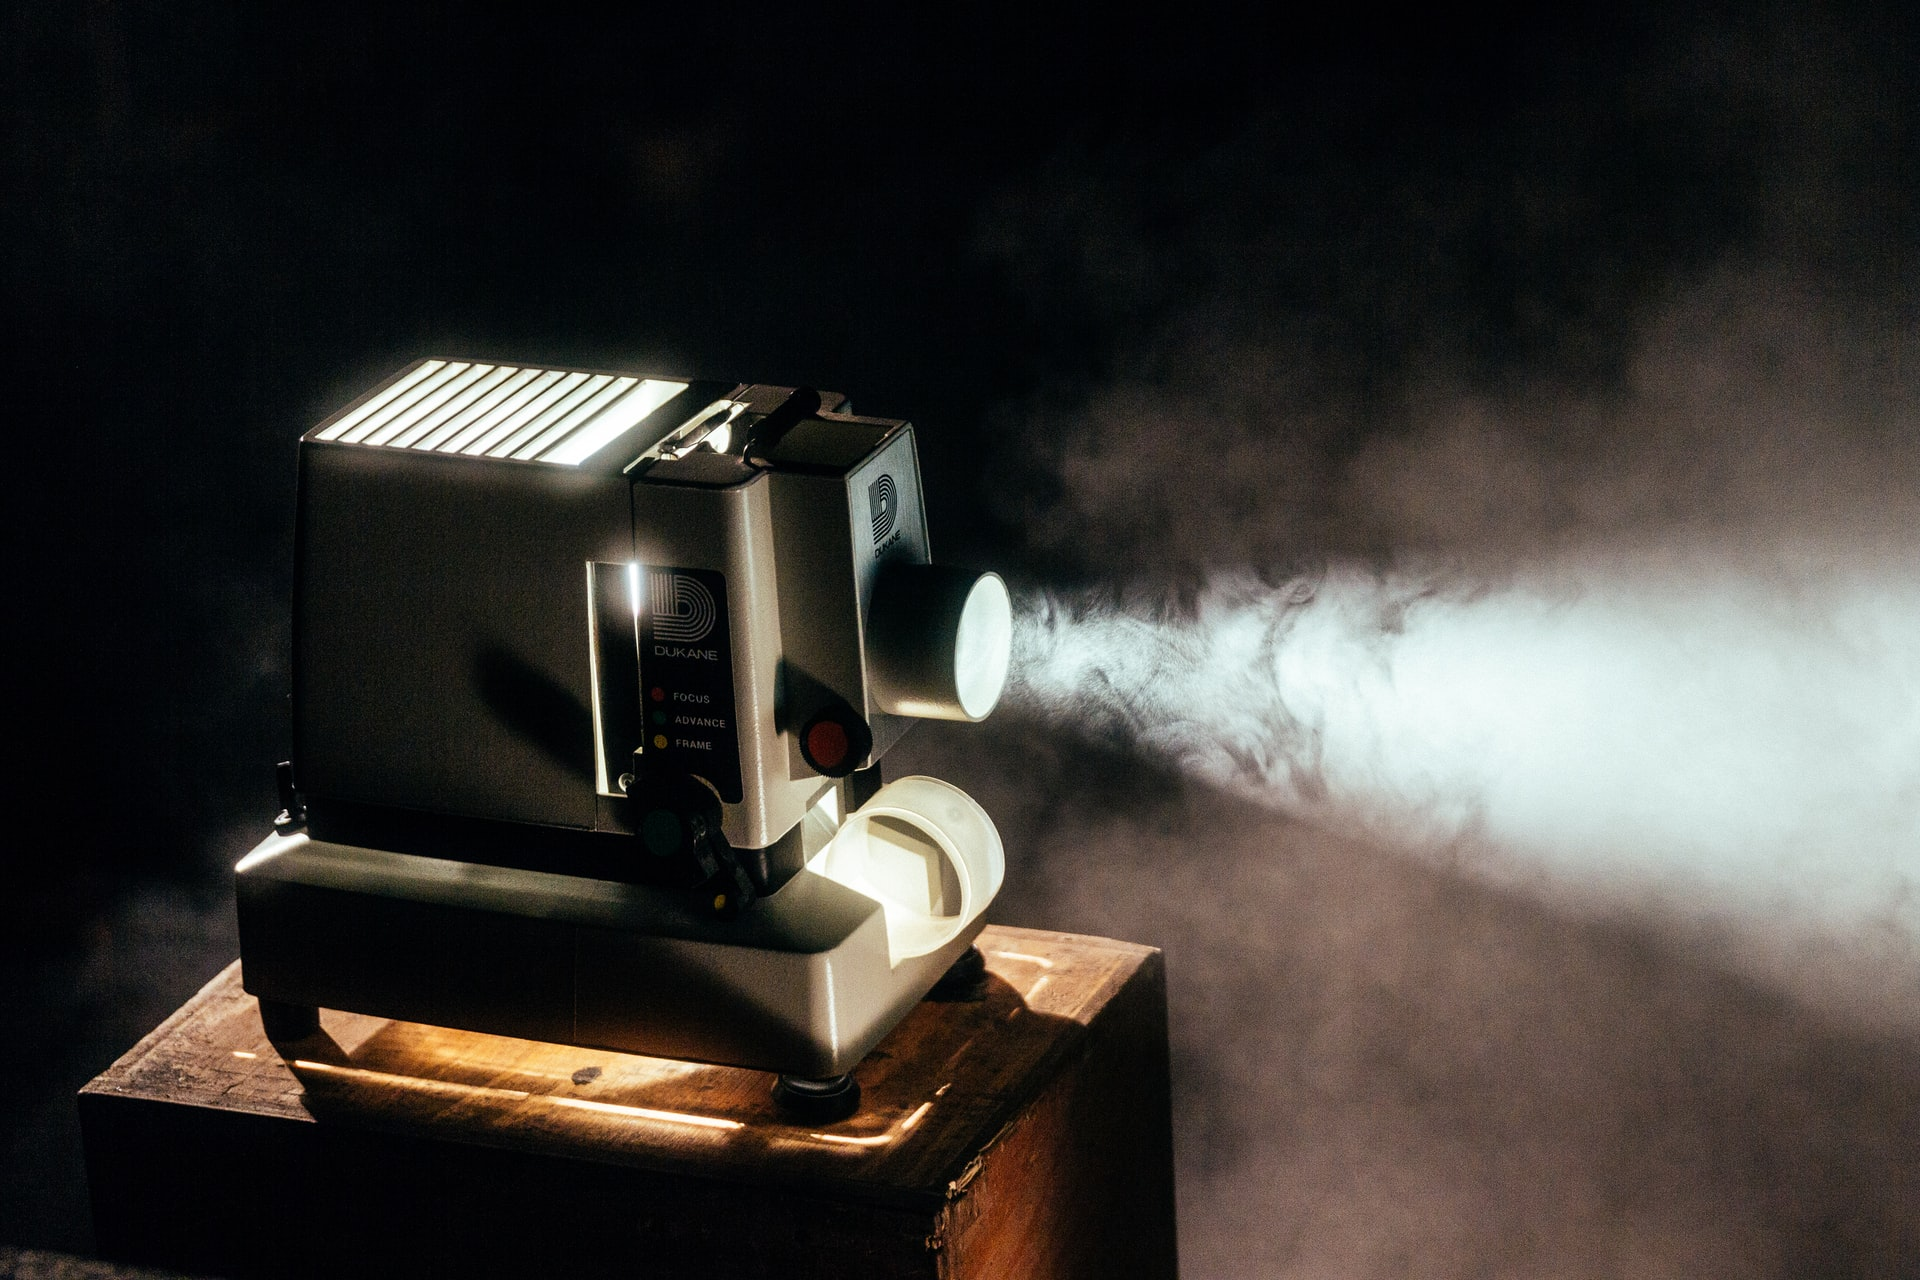
\includegraphics[width=0.8\textwidth]{images/02-projector.jpg}
    \caption{A projector is above all a light emitter. Source: \citet{ImageProjector}}
    \label{fig:background_projector}
\end{figure}

As briefly mentioned in section \ref{section:intro-problem_setting}, no projector is capable of reproducing arbitrary appearance. Each projector can only reproduce a subset of all possible colors, called the \textit{gamut}. Limited projector gamuts have a large impact on how projection mapping is done. To get a better intuition of this impact, we will now explain how a particular type of projector works. We will focus on the so-called Digital Light Processing (DLP) projector which is widely used in cinemas as well as home setups.

\subsubsection{DLP Projectors}
\label{section:background-projection_mapping-projectors-DLP}

Film projectors shine a bright light through film to project its contents onto a screen. But what happens when our movie is digital? What does a DLP projector shine its light through? And what impact does it have on its gamut?

According to \citet{WikiDLP}, DLP projectors project images by filtering the bright white light of their lamp. First, the light goes through a rapidly spinning color wheel which is split into a number of sectors: red, green, blue and sometimes also transparent. At any point, all light from the lamp passes through a single color filter, sending a single-channel image towards the lens. By sending out many single-channel images in rapid succession, however, the projector creates the illusion of sending a three-channel image.

Per-pixel intesities of this single-channel image which form its content are controlled by the Digital Micromirror Device (DMD). This device is divided into many tiny mirrors which roughly correspond to individual pixels of the projected image. Each of these mirrors can either reflect light from the color wheel directly into the lens, or into a heat sink which absorbs it and does not let it through. This allows the projector to turn pixels off and on. Grayscales (pixel intensities between full and zero) are produced by rapidly toggling the mirror between the lens and the heat sink. If, for example, a pixel is on 50\% of the time and off 50\% of the time, the resulting intensity is exactly between full and zero.

\begin{figure}[ht]
    \centering
    \begin{subfigure}[b]{0.49\textwidth}
        \centering
        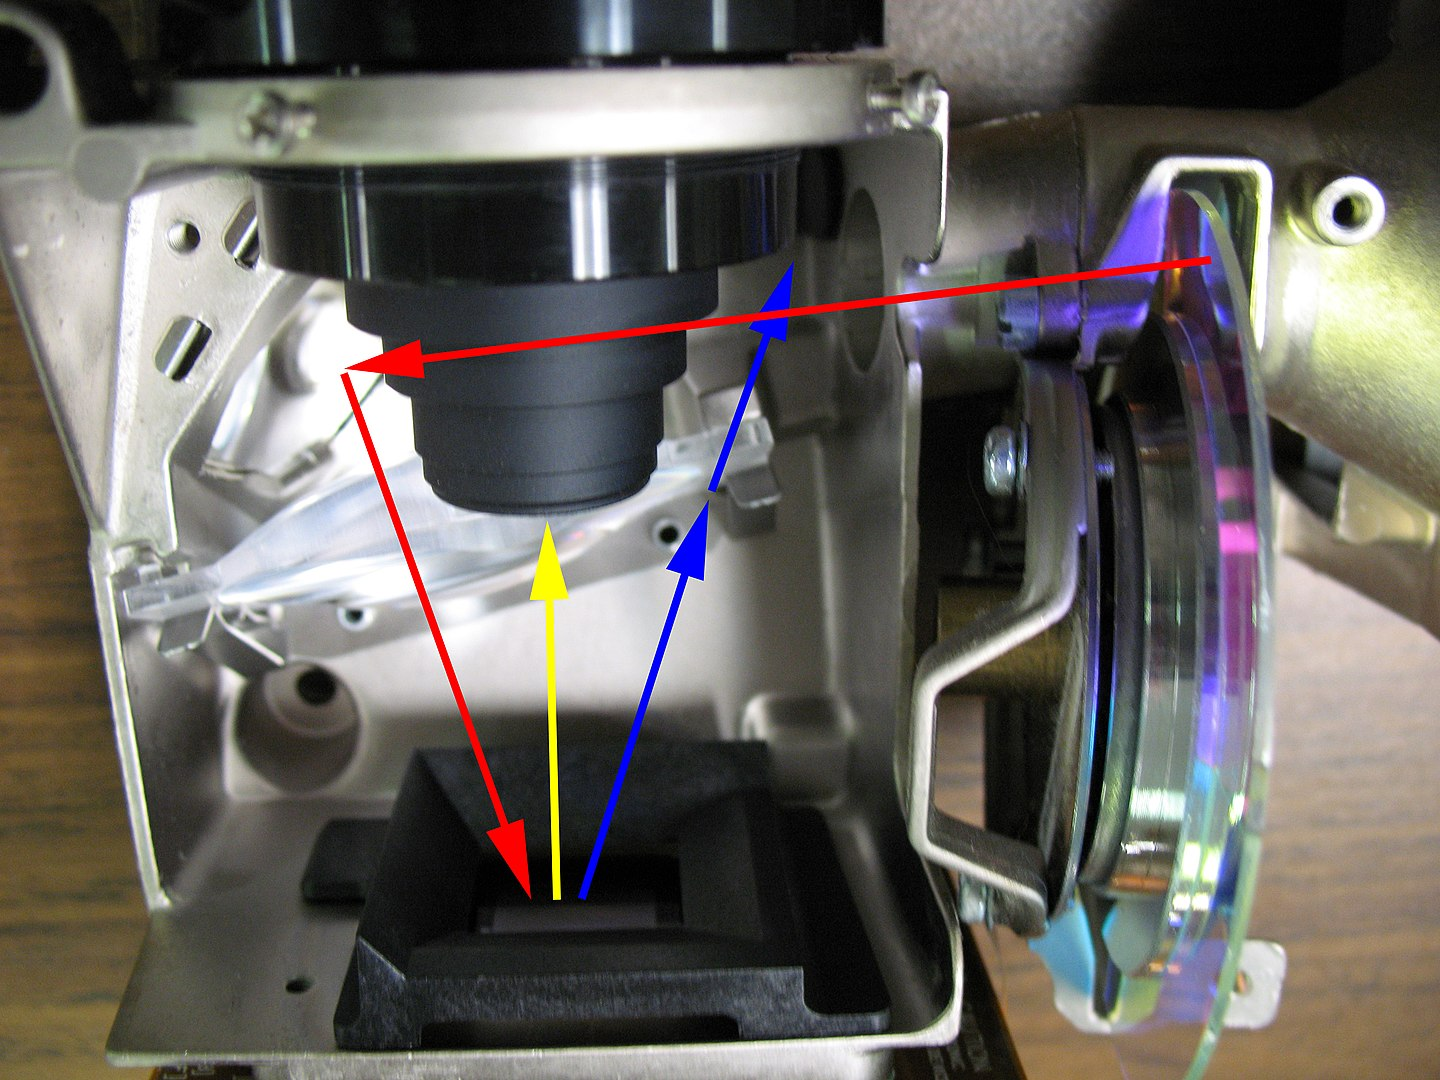
\includegraphics[width=\textwidth]{images/02-projector_dlp.jpg}
        \caption{Source: \citet{ImageProjectorDLP}}
        %\label{}
    \end{subfigure}
    \hfill
    \begin{subfigure}[b]{0.49\textwidth}
        \centering
        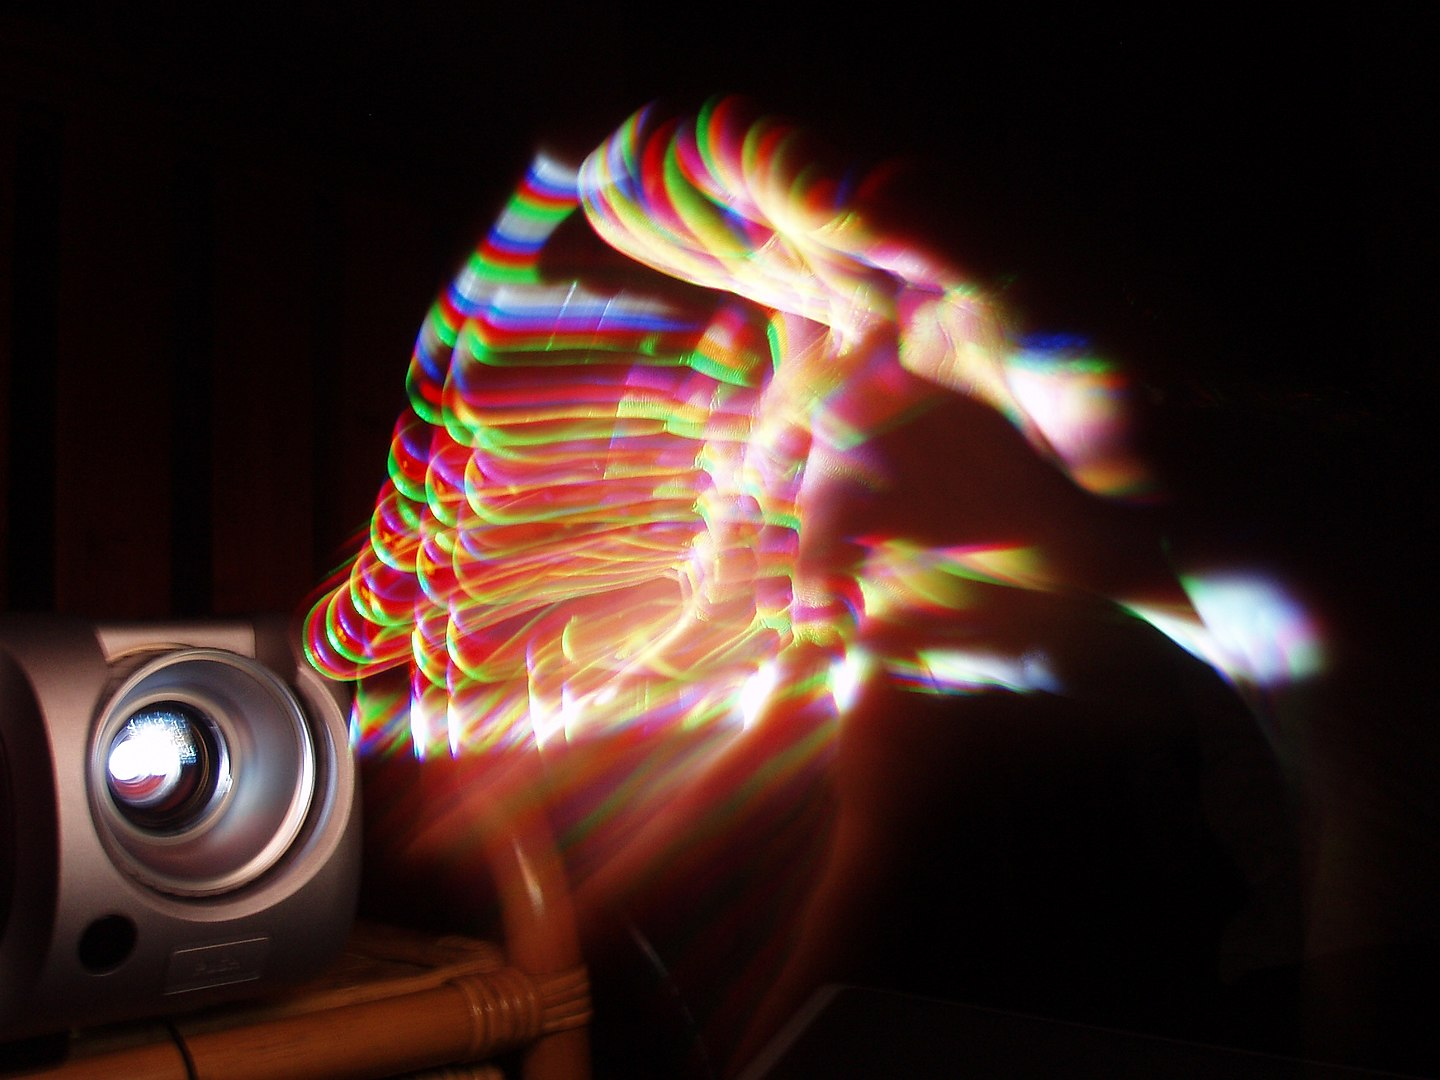
\includegraphics[width=\textwidth]{images/02-projector_rainbow.JPG}
        \caption{Source: \citet{ImageProjectorDLPRainbow}}
        %\label{}
    \end{subfigure}
    \caption{Image a) shows how a DLP projector works. First, bright white light passes through the color wheel. Then it is reflected off the the DMD (red arrows) into either the lens (yellow arrow), or the heat sink (blue arrows). Image b) shows how a DLP projector with a single DMD chip sends out single channel images in rapid succession. This can result in artifacts which can be fixed by using a separate DMD chip for each primary color}
    \label{fig:background_projector_dlp}
\end{figure}

\subsubsection{Hardware Limitations}
\label{section:background-projection_mapping-projectors-limitations}

Based on the way DLPs work, it is easy to see that the process of projecting an image is fairly inefficient and limiting, especially when it comes to the maximum brightness and minimum brightness (also known as black level) of a projector.

Maximum brightness is simply limited by the brightness of the lamp. The brighter the lamp, the more energy it consumes and the more energy is wasted when dark colors or blacks are being projected.

Minimum brightness is related to the ability of the projector to absorb light which is not reflected directly towards the lens. The more light is absorbed inside the projector, the more the projector heats up. This is why DLP projectors with deep blacks need to be large enough to cool themselves down efficiently. If a DLP projector is not able to absorb all the light, some of it is let through towards the screen and is visible as dim gray instead of black.

Different projector technologies have different limitations. For example laser projectors are generally more efficient and brighter because they produce exactly the light color which is needed, as opposed to filtering out white light. But even laser projectors cannot be infinitely bright and even a projector which can produce true black color will not be able to project it onto scenes under external illumination.

An important thing to keep in mind when projecting onto screens, but especially crucial for projection mapping, is that it is impossible to reproduce arbitrary appearance. The less of a particular color a given background reflects, the more difficult it is to project that color onto it.

\subsection{Intuition on Projection Appearance}
\label{section:background-projection_mapping-projection_intuition}

To study projection apperance rigorously, we need light transport theory which we present in the following section. First, however, we believe it is useful to provide the reader with an intuition on what to expect when we install a projector and press Play.

The appearance of an object is given by the light it reflects. Light is the visible portion of electromagnetic radiation and consists of photons at various wavelengths. Wavelengths which human vision is sensitive to are approximately between 380 and 780 nm (\citet{PBRT3e}). Shorter wavelengths appear blue, middle ones are green and longer ones are red. Reflectance of an object is defined by the so-called \textit{spectral power distribution} (SPD) which describes what proportion of incoming light is reflected at each wavelength.

{\color{red} TODO: figure of reflectance of lemon peel from PBRT}

Projectors are then nothing but light sources. As a matter of fact, each of the millions of tiny mirrors inside the DMD of a DLP projector can be thought of as a separate light source. Projector light has an SPD of its own, describing how much power it carries at each wavelength. When it interacts with a surface, something roughly corresponding to SPD multiplication takes place. If an objects does not reflect any light at 450 nm, all of it will be absorbed and will not reach our eyes.

See figure for examples of how projection interacts with various backgrounds.

{\color{red} TODO: figure of projection interacting with various backgrounds}

We will now study this process more carefully using light transport theory.

\subsection{Light Transport Theory}
\label{section:background-projection_mapping-light_transport}

Light transport theory is the study of how things look. This depends on a number of variables, such as object geometry and materials, light sources and a point of view. The most common application of this theory can be found in rendering, for example of architectural visualizations or video games. There, a scene is given along with a camera view and the goal is to compute what is visible and how it looks. Our case is very similar. We have a scene with a projector (i.e. a light source) and our goal is to predict what the scene will look like from a point of view that focuses on the projection. Once we know that, we are only a step away from controlling the projection in a way that the scene looks exactly the way we want -- from projection mapping.

In this section, we provide a brief overview of light transport theory. For a more comprehensive coverage, we refer the reader to our source, Physically Based Rendering: From Theory to Implementation by \citet{PBRT3e}.

\subsubsection{Radiance}
\label{section:background-projection_mapping-light_transport-radiance}

As mentioned in \ref{section:background-projection_mapping-projection_intuition}, all we see is light. Measuring light is therefore the crux of understanding how things look. The fundamental quantity we are interested in is \textit{radiance}. It is defined as the amount of photons \(Q\) per unit projected area \(A^\perp \) per unit solid angle \(\omega\) per unit of time \(t\):

\begin{equation}
    \label{eq:radiance}
    L = \frac{dQ}{dA^\perp d\omega dt}
\end{equation}

{\color{red} TODO: figure of radiance}

{\color{red} TODO: mention that radiance is wavelength-dependent and how this is handled in our equations?}

{\color{red} TODO: mention luminance?}

We will now present the relationship between objects, light sources and the radiance incoming onto our camera sensor or eye retina. This relationship is called the \textit{rendering equation}.

\subsubsection{Rendering Equation}
\label{section:background-projection_mapping-light_transport-rendering_equation}

The rendering equation describes the amount of outgoing radiance from point \(x\) in a scene towards a direction \(\mathbf{v}\):

\begin{equation}
    \label{eq:rendering_equation}
    L(x \rightarrow \mathbf{v}) = \int_{\Omega(x)} L(x \leftarrow \mathbf{u}) f_r(x, \mathbf{u} \rightarrow \mathbf{v}) \cos \theta d\mathbf{u} + E(x \rightarrow \mathbf{v})
\end{equation}

{\color{red} TODO: figure of rendering equation}

where \(L(x \leftarrow \mathbf{u})\) is the radiance arriving at \(x\) from direction \(\mathbf{u}\), \(\Omega(x)\) is the hemisphere oriented to the direction of the surface normal at \(x\), \(f_r\) is the spatially-varying bidirectional reflectance distribution function (SVBRDF) which determines surface reflectance for each point \(x\), incoming direction \(\mathbf{u}\) and outgoing direction \(\mathbf{v}\), and \(\theta\) is the angle between \(u\) and the surface normal at \(x\). Finally, \(E(x \rightarrow \mathbf{v})\) is the radiance emitted from \(x\) towards \(\mathbf{v}\) in case \(x\) lies on a light source.

The main idea of the equation is that radiance leaving towards \(\mathbf{v}\) from \(x\) is the sum of reflected and emitted radiance. It assumes empty space between objects, therefore no light scattering occurs between them. This means that radiance is constant along straight lines and the equation is recursive -- \(L(x \leftarrow \mathbf{u}) = L(y \rightarrow -\mathbf{u})\) where \(y\) is the point seen from \(x\) in the direction of \(\mathbf{u}\).

Apart from assuming that our objects are in vacuum, the equation also assumes that light is reflected from the same point it arrived at. This is generally not the case as can be seen for example with human skin where light under the surface before it is reflected. Both subsurface scattering and participating media are handled in modern renderers which generalize the rendering equation to account for these phenomena ({\color{red} TODO: reference papers that do that?}). For our purposes, however, it is sufficient to be familiar with the basic form of the rendering equation.

\subsubsection{Towards Projection Mapping}
\label{section:background-projection_mapping-light_transport-towards_projection_mapping}

What is the difference between rendering and projection mapping and what makes projection mapping so challenging? In rendering, Monte Carlo integration is often use to solve the rendering equation and thus determine the amount of radiance reflected towards the camera. Scene geometry, materials and the positions and properties of light sources are known ({\color{red} TODO: figure?}). In projection mapping, we do know the amount of radiance that is reflected towards the camera -- it is our desired appearance of the scene. However, everything else is unknown. From scene geometry and materials to the source of the radiance -- the projection image ({\color{red} TODO: figure?}).

Projection mapping algorithms therefore do not typically solve the full light transport of the whole scene, but instead they build on top of assumptions, such as ({\color{red} TODO: 1-2 assumptions}), and provide estimates. We shall now review some of the common approaches to projection mapping found in state-of-the-art methods.

\subsection{Projector-Camera Systems}
\label{section:background-projection_mapping-procams}

The key idea in projection mapping is to use a camera to observe the projection and provide information on how to adapt it to achieve desired appearance. This system as a whole is called the \textit{projector-camera system}, commonly shortened as \textit{procam}.

As mentioned in section \ref{section:background-projection_mapping-light_transport-towards_projection_mapping}, general projection mapping, or solving full light transport in a scene where the only known quantity is radiance arriving at the camera sensor, is very challenging and simplifying assumptions are therefore needed to make the problem tractable. One such assumption is that each camera pixel is influenced by exactly one projector pixel, or at most by a small neighborhood around that pixel. Although this is not the case for example when light bounces around the scene multiple times, methods that use this assumption are reasonably general.

Methods that assume 1:1 pixel correnpodencies between camera and projector are usually split into two parts: \textit{geometric calibration} and \textit{radiometric calibration}. The goal of geometric calibration is to determine those correspondencies. Once we know which projector pixels affect which camera pixels, and therefore the pixels of our desired appearance, we need to find our \textit{how} they affect them. This is done using radiometric calibration which determines the relationship between the intensities of each pair of corresponding projector and camera pixels.

{\color{red} TODO: doesn't this implicitly require per-pixel matching? investigate and explain the consequences this would have for our method!}

Methods that try to account for global illumination effects typically use different assumptions to make the problem tractable, for example that a scene can only be composed of Lambertian objects of constant color ({\color{red} TODO: cite example (Siegl, 17?)}). Those that do attempt to solve general light transport take several hours to calibrate provide only an approximate solution which can only account for some global illumination effects ({\color{red} TODO: cite example (Wetzstein, 07)}).

We will now briefly cover a few methods that rely on geometric and radiometric calibration and one method that attempts to solve general light transport. For a complete overview of the state of the art in projection mapping, see \citet{Grundhofer2018}. We have chosen the methods we are about to describe for the following reasons:

\begin{itemize}
    \item To show that even the latest methods working in simplified scenarios without global illumination effects are severly limited by projector hardware
    \item To show how general light transport can be solved with procams what the challenges when taking this approach are ({\color{red} TODO: tie it together with the LT matrix stuff you're doing later on})
\end{itemize}

\subsubsection{Geometric Calibration}
\label{section:background-projection_mapping-procams-geometric_calibration}

The goal of geometric calibration is to find a point \(M_c = [u_c, v_c]^T\) in the camera image for each point \(M_p = [u_p, v_p]^T\) in the projector image such that the value of the latter determines the value of the former. These correspondencies are usually established via a third point, \(P = [x, y, z]\) which is located in the scene.

The relationship between \(M_c\) and \(P\) is determined by the \textit{intrinsic} and \textit{extrinsic} matrices:

\begin{equation}
    \label{eq:camera_equation}
    \begin{bmatrix}
        M_c \\
        1
    \end{bmatrix} =
    \begin{bmatrix}
        f_x & c & u \\
        0 & f_y & v \\
        0 & 0 & 1 
    \end{bmatrix} \cdot
    \begin{bmatrix}
        \mathbf{R} & \mathbf{t}
    \end{bmatrix} \cdot
    \begin{bmatrix}
        P \\
        1
    \end{bmatrix}
\end{equation}

{\color{red} TODO: fix the matrix, so that the dimensions check out}

where the intrinsic matrix is formed by camera focal lengths \(f_x\) and \(f_y\) (there are two focal lengths because they are expressed in camera pixels which are generally rectangular), skewness \(c\) of image axes, and principal point coordinates \([u, v]^T\) (the intersection of optical axis and image plane which is generally not in the center of the image). The extrinsic matrix is then formed by rotation \(\mathbf{R}\) and translation \(t\) which convert between world coordinates and camera coordinates.

The most commonly used method for finding the parameters of \ref{eq:camera_equation} was introduced by \citet{Zhang1999}. They are estimated by taking at least two photos of a planar pattern at various orientations.

We will now outline two recent methods to perform geometric calibration. The first one requires user assistance, while the second one is fully automatic.

\textbf{One camera, one projector and a calibration board.} The first method, introduced by \citet{Yang2016}, uses a calibration board containing a random dot pattern. First, the camera is calibrated using the approach of \citet{Zhang1999}. Then the projector is calibrated by projecting another dot pattern onto the board using the inverse camera method. The whole process needs around 10 views of the calibration board according to experiments in the paper.

\textbf{Two cameras, one projector.} An entirely automatic self-calibration method was presented by \citet{Willi2017}. Their method first establishes pixel correspondencies between the two cameras and then continues to estimate the intrinsic and extrinsic matrix, as well as the 3D point cloud of the scene. Finally, the projector is calibrated using this information. It is worth noting that this method works also for any larger number of projectors and cameras in which case camera pairs are sorted by the quality of their pixel correspondencies. Calibration is first done for the best pair and other devices are incorporated iteratively, improving the overall estimate.

Both methods work only on static scenes and take several minutes to complete. Real time methods also exist, but those usually rely on some prior knowledge about scene geometry ({\color{red} TODO: find example}) or on time-consuming pre-calibration followed by incremental updates ({\color{red} TODO: find example}).

{\color{red} TODO: assumptions on diffuse surfaces that make the correspondencies 1:1?}

\subsubsection{Radiometric Calibration}
\label{section:background-projection_mapping-procams-radiometric_calibration}

Once correspondencies between projector and camera pixels have been established using one of the methods described in section \ref{section:background-projection_mapping-procams-geometric_calibration}, radiometric calibration can be performed. In general, the goal is to find a color-mapping function \(f\) such that

\begin{equation}
    \label{eq:radiometric_calibration}
    c_c = f(c_p)
\end{equation}

where \(c_c\) is the color of a camera pixel and \(c_p\) is the color of the corresponding projector pixel. We describe one method that assumes \(f\) to be linear and one method that allows for arbitrary \(f\).

\textbf{Linear color-mapping function.} One of the first projection mapping methods was presented by \citet{Grossberg2004}. There, the relationship between \(c_c\) and \(c_p\) is specified as follows:

\begin{equation}
    \label{eq:linear_color_mapping}
    c_c = p_c(V p_p(c_p) + F)
\end{equation}

where \(p_p\) is a non-linear projector response function which turns input pixel values into projector brightness, \(p_c\) is a non-linear camera response that converts radiance arriving at the camera sensor to an output pixel value, \(F = [F_R, F_G, F_B]\) is the environment light term which is independent of the projector, and finally \(V\) is a \(3 \times 3\) color mixing matrix which captures the relationship between projector and camera channels and their interactions with spectral reflectance.

{\color{red} TODO: tidy up the notation}

Both \(p_p\) and \(p_c\) are independent of the scene and can be estimated separately. \(V\) and \(F\) are per-pixel and scene-dependent and can be estimated by projecting and capturing 6 calibration images.

The disadvantage of this method are that the linear color mixing matrix is not an accurate model for example when using DLP projectors described in section \ref{section:background-projection_mapping-projectors-DLP}. DLP projectors sometimes form an image by composing red, green, blue and white channels together. The extra white channel may result in non-linear behavior. Another disadvantage is that if the color gamut of the projector struggles to reproduce color required by the compensation model, it results in clipping artifacts and lowered contrast {\color{red} TODO: verify this precisely}.

\textbf{Non-linear color-mapping function with a global optimization step.} To solve these problems, \citet{Grundhofer2015} presented an improved method which allows for an arbitrary color-mixing function. This function is estimated by obtaining up to \(6^3\) samples and then applying thin-plate spline interpolation on these samples. This sampling process takes several minutes but once it is completed, compensation can be performed in real time.

On top of that, the paper also introduces an important idea ({\color{red} TODO: it has been used before, though\dots}) of content-based projection image compensation. This is a separate step which can also take several minutes and consists of optimizing per-pixel (or per-patch) coefficients which scale the final luminance values of the image. The goal of this optimization is to minimize clipping errors cause by limited color gamut of the projector and overall increase image contrast.

As a result, this method achieves very good results in scenes which have minimal inter-reflection that cannot be modeled when 1:1 correspondence between projector and camera pixels is assumed. The idea of the global optimization step is also very important for our thesis because it suggests that algorithms that try to optimize the L2 distance between camera image and desired appearance do not always yield the best-looking results.

{\color{red} TODO: modify the intro to the thesis to make it clear that content-based compensation is an old idea as such}

\subsubsection{Inverse Light Transport}
\label{section:background-projection_mapping-procams-inverse_lt}

If the goal of light transport is to compute what a scene looks like based on its illumination (among other things), then the goal of inverse light transport is to compute how a scene is illuminated based on what it looks like. This is the most general formulation of the projection mapping problem since it does not split the problem into geometric calibration and radiometric calibration, but instead looks at it as a whole.

\citet{Wetzstein2007} present a method for projection compensation via inverse light transport. They start from the observation that light transport is linear. This means that if there are two light sources in a room and two photos of it were taken, one with only one light on and the other with only the other light on, then taking a linear combination of the photos would yield a correct photo of the room with the same combination of the two lights on ({\color{red} TODO: figure would be nice, also better worded sentence would help. derive it from the rendering equation maybe?}). As a consequence, light transport can be determined by a matrix \(A\):

\begin{equation}
    \label{eq:lt_matrix}
    A = \begin{bmatrix}
        c_{11} & c_{21} & c_{31} & \dots & c_{m1} \\
        c_{12} & c_{22} & c_{32} & \dots & c_{m2} \\
        c_{13} & c_{23} & c_{33} & \dots & c_{m3} \\
        \vdots & \vdots & \vdots & \ddots & \vdots \\
        c_{1n} & c_{2n} & c_{3n} & \dots & c_{mn}
    \end{bmatrix}
\end{equation}

where \(m\) is the number of light sources in a scene, \(n\) is the number of pixels in the camera sensor and \(c_{ij}\) is the value of the \(j\)-th pixel of an image that was rendered with only the \(i\)-th light source turned on. By taking a linear combination of the columns of the matrix it is then possible to obtain an image rendered by the corresponding combination of light sources.

In projection mapping, this matrix is usually extremely large because \(n\) corresponds to camera resolution and \(m\) corresponds to projector resolution. In colorful images, each \(c_{ij}\) is then a 3-dimensional vector. The two main challenges are therefore to

\begin{enumerate}
    \item Capture the matrix
    \item Obtain its inverse
\end{enumerate}

In practice, it is impossible to capture the matrix by projecting a canonical basis because this would mean projecting with only a single pixel turned on and the signal-noise ratio of camera sensors is too high to capture such faint light. There exist several methods to capture the light transport matrix, such as ({\color{red} TODO: examples}). Most of these methods use the fact that the matrix is very sparse in practice. In fact, the less inter-reflection there is in a scene, the sparser the matrix is. \citet{Wetzstein2007} use ({\color{red} TODO: cite the method they use}) which can still take up to several hours. Moreover, the matrix has to be captured again when the scene or projector position changes.

It is also practically impossible to invert such a large matrix. \citet{Wetzstein2007} therefore estimate its pseudo-inverse. The drawback of this approach is that some global illumination illumination information is lost, such as projector defocus, and therefore the compensation is not accurate.

The benefit of this method is, however, that it does not make any assumptions about surface material and works well even with glass and mirrors which are impossible to project on using other methods.

({\color{red} TODO: bridge to synthesis? also, why did you talk about this method?})

\section{Texture Synthesis}
\label{section:background-texture_synthesis}

As mentioned in section \ref{section:intro-key_idea}, the aim of this thesis is to advance the idea of content-based projection mapping of textures. If, as section \ref{section:background-projection_mapping} suggests, it is very difficult with current projector hardware to find a compensated projection image such that its pixel values are are close as possible to the desired appearance while minimizing clipping errors, maybe it is a good idea to loosen up the definition of image similarity. Textures are a great candidate for that because two textures can have radically different pixel values in corresponding position but still look the same.

{\color{red} TODO: example of two images that are different but show the same texture}

But what exactly is a texture and what kind of image modifications can be done while preserving it? In this section, we provide an overview of texture synthesis research which is the second building block that our method relies on.

\subsection{Textures}
\label{section:background-texture_synthesis-textures}

{\color{red} TODO: mention the Texture Hypothesis by Julesz (texture is defined by 2nd order co-occuring stationary statistics) here}

{\color{red} TODO: provide the deeper theory that used to be in the intro, but isn't anymore}

What is a texture? \citet{Julesz1995}, a prominent visual neuroscientist of the 20th century, has defined textures as classes of images that cannot be discriminated in preattentive vision, i.e. by quickly glancing over them. This definition implies that any algorithm that claims to synthesize different textures of a given class can only be evaluated empirically. Work has gone into creating models that would describe what constitues a texture class and thus help in developing synthesis algorithms and evaluating them. No single model has, however, emerged as clearly superior thus far. Each synthesis method typically defines its own model and even if convergence under such a model is proved, the quality of the results is ultimately up to the observer.

In general, two approaches to texture synthesis have emerged. One is inspired by \citet{Shannon1948} and his use of a Markov chain to generate English text. There, each letter is sampled from a probability distribution conditioned on \(n\) previous letters. The result is not precisely English text, but rather a "texture" of it. ({\color{red} TODO: show example?}) \citet{Efros1999} have built on this idea by introducing a way to synthesize textures pixel by pixel where each pixel is conditioned on the previous ones. \citet{Raad2018} call this approach \textit{patch re-arrangement} or \textit{patch-based texture synthesis}.

The other approach has been pioneered by Julesz himself and relies on statistical descriptions of images such that if two different images share this description, they are the same texture. Already in 1973, \citet{Julesz1973} observed that certain texture pairs cannot be discerned by human preattentive vision if they share the same second-order statistics. Building on this idea, \citet{Galerne2011} have presented a method that creates a new example of the same texture by randomizing its Fourier phase ({\color{red} TODO: explain what it is}). \citet{Raad2018} call this approach \textit{statistics-based texture synthesis}.

We now discuss patch-based and statistics-based methods in more detail to find out what their strenghts and weaknesses are and how they could be used to generate content-based projection compensations.

\subsection{Patch-Based Texture Synthesis}
\label{section:background-texture_synthesis-patch_based}

\citet{Efros2001} have presented a simple but powerful method called \textit{image quilting} for texture synthesis using patch re-arrangement. They start by splitting the input texture image into overlapping square blocks \(B_i\) of size \(k\) which is a user-controlled parameter. Then they build the new texture block by block in raster scan order (from the top left corner to the bottom right corner, row by row). A new block \(B^{\prime}\) is chosen at random from all \(B_i\) such that the pixel-wise error in overlapping areas (they use 1/6 of block area along the edge) with the block above \(B^{\prime}\) and to the left of \(B^{\prime}\) in below a certain threshold in the output image. Since many blocks usually satisfy this overlap constraint, one is picked at random. If \(B^{\prime}\) was pasted into the output image directly, the result would look blocky. Therefore \(B^{\prime}\) is pasted into the output image along a minimum error path inside the overlapping areas. This ensures that seams between block will be as subtle as possible.

({\color{red} TODO: figure to illustrate the algorithm, especially the minimum error path!})

\subsubsection{Pros and Cons}
\label{section:background-texture_synthesis-patch_based-pros_and_cons}

This method can achieve stunning visual results when the input texture is uniformly lit and contains large features, like pebbles or coffee beans. It is especially powerful when used on textures with regular structure, like a brick wall.

However, it struggles with textures that have non-uniform illumination and that contain very small features, like sand or concrete. Failure cases usually manifest themselves by large areas that are directly copied from the input (so-called \textit{verbatim copying}) or areas that contain the same patch copied over and over (so-valled \textit{garbage growing}).

Another drawback of this method is that its parameters need to be manually tuned based on the feature sizes and other properties of the input texture. There is also no underlying texture model that this method would work with which means that reasoning about it is somewhat less robust and limited to measuring heuristics such as the amount of verbatim copies and garbage in the output.

\subsubsection{Potential Usage in Projection Mapping}
\label{section:background-texture_synthesis-patch_based-projection_mapping}

Image quilting is surprisingly flexible to adapt for other uses than texture synthesis. The authors themselves showcase the possibility of using the method for style transfer. This is a problem that considers two input images and produces a third one which has the content of one image and style of the other.

({\color{red} TODO: example!})

This can be achieved by adding a new term to the overlap error. In the case of style transfer, this takes the form of the difference in luminance values of corresponding pixels in the input and output images.

One could imagine modifying the method to achieve projection mapping. If the output image was the compensated projection image the additional error term might be inversely proportional to how far the pixel value in the output is to the limit of the color gamut of the projector once it is radiometrically compensated. This could be built on top of methods such as \citet{Grundhofer2015} that assume 1:1 correspondence between projector image and camera image. ({\color{red} TODO: explain better\dots})

\subsection{Statistics-Based Texture Synthesis}
\label{section:background-texture_synthesis-statistics_based}

All statistics-based methods for texture synthesis share the general workflow. They first extract a set of statistics from the input texture image. Then they initialize a random noise image and iteratively optimize it so that its statistics are the same as those of the input image ({\color{red} TODO: figure}). Different initializations of the noise image yield different final results (unless the statistics are too restrictive so as to represent only one image) and by computing the difference between the statistics of the input and the output we can easily argue about convergence of such methods.

\citet{Gatys2015} have introduced a breakthrough method for statistics-based texture synthesis which significantly improved over the previous state of the art. This method relies on a \textit{convolutional neural network} (CNN) to produce a statistical description of a texture image that the noise initialization is then optimized to fit. Let us first briefly introduce what a CNN and what makes it so powerful at creating abstract descriptions of images.

\subsubsection{Convolutional Neural Networks (CNNs)}
\label{section:background-texture_synthesis-statistics_based-cnns}

\textit{Neural networks}, or more precisely \textit{feedforward neural networks}, are essentially functions

\begin{equation}
    \label{eq:neural_network}
    y = f(x, \phi)
\end{equation}

where \(x\) is the input, \(y\) is the output and \(\phi\) are the parameters of a neural network. The idea is that \(f\) is an approximation of \(f^\star\) which is a very complex, non-linear function which tells us something about the world. For example, we can consider \(f^\star\) to be the mapping between all possible images of size \(224 \times 224\) and categories such as dog, cat, tree, house, etc. that describe the image. The goal of \textit{deep learning}, which is the study of feedforward and other kinds of neural networks, is then to find an \(f\) along with its parameters \(\phi\) that approximate \(f^\star\) as closely as possible. Because of the complexity of \(f^\star\), \(f(x) = f^{(3)}(f^{(2)}(f^{(1})(x)))\) is often composed of many functions \(f^{(i)}\) which are called \textit{layers}. Each layer usually operates on vectors and is commposed of small units that are loosely modeled on brain neurons. Together, these layers form a network where information flows from the first layer to the last. Hence the term \textit{feedforward neural network}.

{\color{red} TODO: mention training?}

Convolutional neural networks (CNNs) form a class of neural networks that are intended for processing grid-like inputs, for example images (2D grid) or audio (1D grid). Their layers are typically composed of three parts: convolution, nonlinearity and pooling.

{\color{red} TODO: image}

\textbf{Convolution}. To explain convolution in the context of neural networks, it is best to start with an example. Let us imagine that we have an image and would like to find all vertical edges in that image. This can be done using convolution ({\color{red} TODO: image}). All we need to do is take a \(3 \times 3\) matrix ({\color{red} TODO: figure out the right values\dots}), also called \(kernel\), move it across the image aligning the center of the kernel with each image pixel in turn, multiplying overlapping values, summing them together and writing them out into a new image. We will notice that the new image contains high values in places where there is a vertical edge in the original image. What has happened?

The process we have gone through with our image and our kernel is called convolution in the context of deep learning, although strictly speaking, it corresponds to cross-correlation which differs from convolution by the orientation of the kernel. Our kernel happens have values which detect vertical edges when convolved with an image. Kernels with different values do different things, for example detect horizontal edges, blur the image, or even leave it untouched ({\color{red} TODO: examples!}).

Kernel values are what constitutes the parameters \(\phi\) of a CNN and it turns out that they are powerful enough to achieve impressive results in tasks such as object recognition, ({\color{red} TODO: more examples}). They cannot function alone, however. As we have mentioned, neural networks usually approximate complex non-linear function and convolutions as presented here are linear. Two more building blocks are therefore needed.

\textbf{Nonlinearity}. Nonlinearities are scalar functions whose purpose is to simply introduce nonlinear behavior into a CNN. Many types of nonlinearities have been proposed in recent years, for example hyperbolic tangent or ReLU ({\color{red} TODO: figures}). ReLU is used more commonly simply because it improves results ({\color{red} TODO: maybe cite some justification for this?}).

\textbf{Pooling}. Pooling functions are function that accept a vector as input and return a scalar as output. They are often use to make CNNs invariant to small shifts in the input image and also reduce the size of the intermediate outputs, also called \textit{activations}, of each CNN layer. ({\color{red} TODO: a bit more explanation with images?})

CNNs typically have multiple such layers and since they are trained to classify images, the have a few fully connected layers ({\color{red} TODO:  explain?}) at the end which compress the activations into an \(n\)-dimensional vector where each position of the vector corresponds to a particular image class and the value at that position tells how likely the input image is to belong to that image class. For a more comprehensive overview of neural networks and deep learning, see \citet{Goodfellow2016}. We will now focus how CNNs are related to texture synthesis.

{\color{red} TODO: depth of output? number of feature maps? RGB channels?}

{\color{red} TODO: biases?}

{\color{red} TODO: fully connected layers? classification output?}

For texture synthesis as introduced by \citet{Gatys2015}, however, it is only the activations after individual convolution layers that matter. The operation of convolution and the fact that the network is trained to classify images ({\color{red} TODO: deep image prior?}) causes those activations to contain filtered versions of the input image where particular features that define a texture are emphasized ({\color{red} TODO: now it would be great to have a visualization of which features are picked out at which levels!}).

\subsubsection{Texture Synthesis Using CNNs}
\label{section:background-texture_synthesis-statistics_based-synthesis_using_cnns}

As mentioned in \ref{section:background-texture_synthesis-statistics_based}, statistics-based texture synthesis relies on a statistical description of a texture that white noise images are optimized to match. \citet{Gatys2015} use the activations after each pooling layer of the VGG-19 CNN by \citet{Simonyan2014} to define such a description. These activations, however, contain spatial information of where each feature is located in the texture. In order to remove this spatial information, activation are correlated with each other within each layer. Correlated per-layer activations of VGG-19 therefore constitute a set of statistics completely describing a texture.

To synthesize a new example of a given texture, gradient-based loss optimization is used. The loss is defined as a weighted mean square error between the description of the input texture and the image being optimized. The L-BFGS optimizer is used to drive the optimization process ({\color{red} TODO: why is it a good choice?}).

Let us now summarize exactly what constitutes a texture model in \citet{Gatys2015}.

{\color{red} TODO: give the details to be complete. or leave them for appendix?}

\subsubsection{Pros and Cons}
\label{section:background-texture_synthesis-statistics_based-pros_and_cons}

{\color{red} TODO: show some examples from the paper where they compare to Portilla and Simoncelli}

{\color{red} TODO: refer to \citet{Raad2018} for some more pros and cons\dots}

This method of synthesizing textures leads to high-quality results for a large variety of input images. Compared to patch-based synthesis it also provides a texture model, as opposed to a mere algorithm to generate new textures. This makes it easier to reason about and provide theoretical justifications as to why it works.

One disadvantage of this method is that it struggles with regular patterns, unline patch-based methods. It is also fairly sensitive to input and output image resolution {\color{red} TODO: explain this properly}

\subsubsection{Potential Usage in Projection Mapping}
\label{section:background-texture_synthesis-statistics_based-projection_mapping}

This method could be easily adapted to projection mapping if a differentiable rendering function was added to the optimization loop. The idea is to first project initial white noise image onto a scene and then feed the resulting camera image into the CNN and ultimately compare it against the input texture image. The loss gradients would flow through both the CNN and the rendering function and would be used to update the initial image. The result of this process should be an image which once projected looks like a new example of the input texture.